\documentclass[tikz,border=8pt]{standalone}
\usepackage{amsmath,amssymb}
\usetikzlibrary{arrows.meta,calc,decorations.pathreplacing,patterns,shapes.geometric,positioning,shadings}

\begin{document}
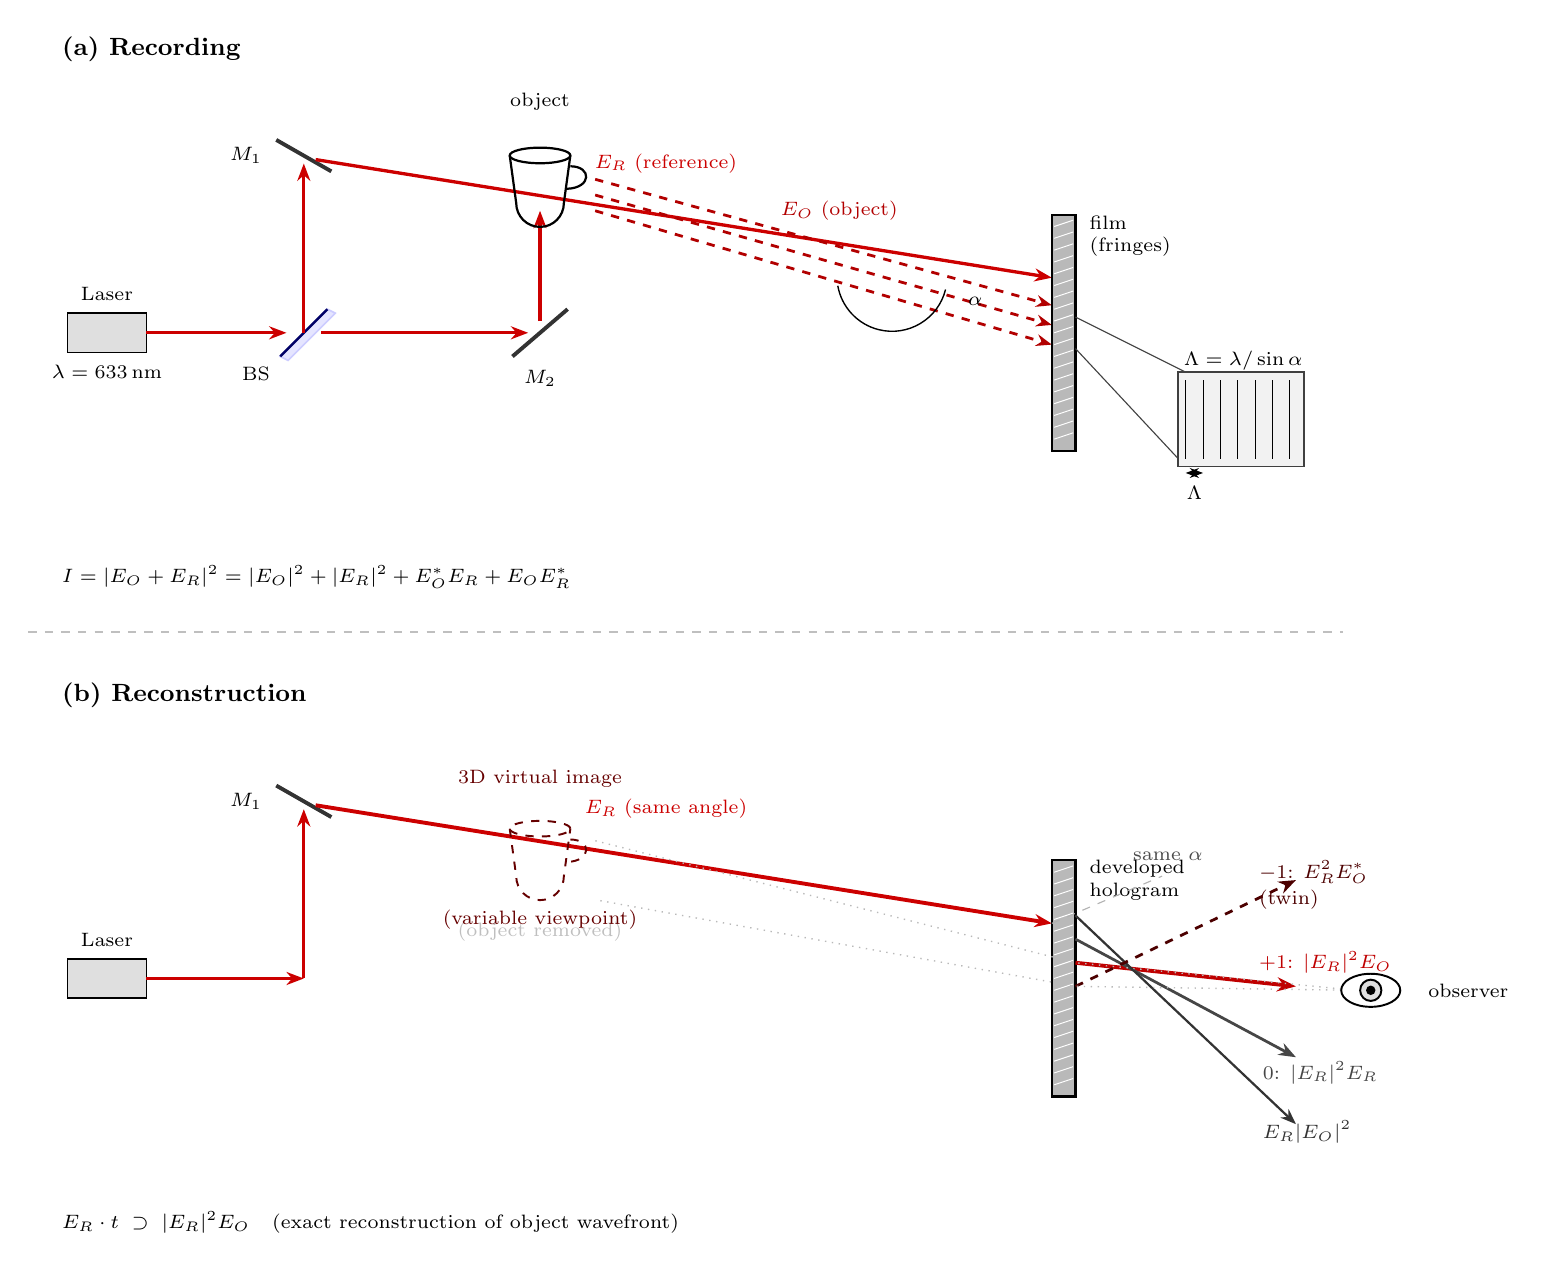
\begin{tikzpicture}[
  >=Stealth,
  thick,
  font=\footnotesize
]

% ==================================================================
% TOP PANEL: Recording stage
% ==================================================================
\begin{scope}[shift={(0,0)}]

  % Panel title
  \node[font=\small\bfseries, anchor=west] at (-7.2,3.6) {(a) Recording};

  % Laser source (left)
  \draw[fill=gray!25, line width=0.6pt] (-7.0,-0.25) rectangle (-6.0,0.25);
  \node[font=\scriptsize, anchor=south] at (-6.5,0.28) {Laser};
  \node[font=\scriptsize, anchor=north] at (-6.5,-0.28) {$\lambda = 633\,\mathrm{nm}$};

  % Laser output beam to beam splitter
  \draw[red!80!black, line width=1.2pt, -{Stealth[length=2.2mm]}] (-6.0,0) -- (-4.22,0);

  % Beam splitter at (-4,0), 45 deg
  \draw[blue!20!white, fill=blue!10, line width=0.6pt]
    (-4.3,-0.3) -- (-3.7,0.3) -- (-3.6,0.25) -- (-4.2,-0.35) -- cycle;
  \draw[blue!40!black, line width=0.9pt] (-4.3,-0.3) -- (-3.7,0.3);
  \node[font=\scriptsize, anchor=north east] at (-4.3,-0.3) {BS};

  % Reflected (upward) beam -> mirror M1 at (-4,2.2)
  \draw[red!80!black, line width=1.2pt, -{Stealth[length=2.2mm]}] (-4.0,0) -- (-4.0,2.15);
  % Mirror M1
  \draw[gray!40!black, line width=1.4pt] (-4.35,2.45) -- (-3.65,2.05);
  \node[font=\scriptsize, anchor=east] at (-4.4,2.25) {$M_1$};

  % Beam from M1 to film (rightward, horizontal-ish to hit film at angle alpha)
  \draw[red!80!black, line width=1.2pt, -{Stealth[length=2.2mm]}] (-3.85,2.2) -- (5.50,0.7);
  \node[red!80!black, font=\scriptsize, anchor=south] at (0.6,1.9) {$E_R$ (reference)};

  % Transmitted (through BS) beam -> mirror M2 at (-1.0, 0)
  \draw[red!80!black, line width=1.2pt, -{Stealth[length=2.2mm]}] (-3.78,0) -- (-1.15,0);
  \draw[gray!40!black, line width=1.4pt] (-1.35,-0.3) -- (-0.65,0.3);
  \node[font=\scriptsize, anchor=north] at (-1.0,-0.35) {$M_2$};

  % Beam from M2 upward to object
  \draw[red!80!black, line width=1.2pt, -{Stealth[length=2.2mm]}] (-1.0,0.15) -- (-1.0,1.55);

  % Object: simple teacup (black thin lines)
  \begin{scope}[shift={(-1.0,1.95)}, scale=0.55]
    % Cup body
    \draw[black, line width=0.8pt] (-0.7,0.55) -- (-0.55,-0.55) arc[start angle=180, end angle=360, radius=0.55] -- (0.7,0.55);
    % Cup rim (ellipse top)
    \draw[black, line width=0.8pt] (0,0.55) ellipse (0.7 and 0.18);
    % Handle
    \draw[black, line width=0.8pt] (0.7,0.3) .. controls (1.2,0.3) and (1.2,-0.2) .. (0.62,-0.22);
  \end{scope}
  \node[font=\scriptsize, anchor=south] at (-1.0,2.7) {object};

  % Scattered object wave E_O from object to film
  \draw[red!70!black, line width=1.0pt, dashed, -{Stealth[length=2.0mm]}] (-0.3,1.95) -- (5.50,0.35);
  \draw[red!70!black, line width=1.0pt, dashed, -{Stealth[length=2.0mm]}] (-0.3,1.75) -- (5.50,0.1);
  \draw[red!70!black, line width=1.0pt, dashed, -{Stealth[length=2.0mm]}] (-0.3,1.55) -- (5.50,-0.15);
  \node[red!70!black, font=\scriptsize, anchor=south] at (2.8,1.3) {$E_O$ (object)};

  % Film (dark gray vertical bar)
  \draw[fill=gray!55, line width=0.8pt] (5.5,-1.5) rectangle (5.8,1.5);
  \foreach \y in {-1.35,-1.2,-1.05,-0.9,-0.75,-0.6,-0.45,-0.3,-0.15,0,0.15,0.3,0.45,0.6,0.75,0.9,1.05,1.2,1.35} {
    \draw[white, line width=0.35pt] (5.53,\y) -- (5.77,\y+0.08);
  }
  \node[font=\scriptsize, anchor=west] at (5.85,1.4) {film};
  \node[font=\scriptsize, anchor=west] at (5.85,1.1) {(fringes)};

  % Angle alpha between E_O and E_R at the film
  \draw[black, line width=0.5pt] (4.15,0.55) arc[start angle=-14, end angle=-170, radius=0.7];
  \node[font=\scriptsize, anchor=east] at (4.75,0.4) {$\alpha$};

  % Fringe spacing zoom callout
  \draw[gray!50!black, line width=0.4pt] (5.8,0.2) -- (7.2,-0.5);
  \draw[gray!50!black, line width=0.4pt] (5.8,-0.2) -- (7.2,-1.7);
  \draw[gray!50!black, line width=0.5pt, fill=gray!10] (7.1,-1.7) rectangle (8.7,-0.5);
  \foreach \i in {0,1,2,3,4,5,6} {
    \draw[black, line width=0.3pt] (7.2+\i*0.22,-1.6) -- (7.2+\i*0.22,-0.6);
  }
  \draw[<->, line width=0.4pt] (7.2,-1.78) -- (7.42,-1.78);
  \node[font=\scriptsize, anchor=north] at (7.31,-1.82) {$\Lambda$};
  \node[font=\scriptsize, anchor=west] at (7.05,-0.35) {$\Lambda = \lambda/\sin\alpha$};

  % Formula at bottom
  \node[anchor=west, font=\scriptsize] at (-7.2,-3.1)
    {$I = |E_O + E_R|^2 = |E_O|^2 + |E_R|^2 + E_O^{*} E_R + E_O E_R^{*}$};

\end{scope}

% Separator
\draw[gray!50, line width=0.4pt, dashed] (-7.5,-3.8) -- (9.2,-3.8);

% ==================================================================
% BOTTOM PANEL: Reconstruction stage
% ==================================================================
\begin{scope}[shift={(0,-8.2)}]

  % Panel title
  \node[font=\small\bfseries, anchor=west] at (-7.2,3.6) {(b) Reconstruction};

  % Laser source (left) -- only reference beam, same angle
  \draw[fill=gray!25, line width=0.6pt] (-7.0,-0.25) rectangle (-6.0,0.25);
  \node[font=\scriptsize, anchor=south] at (-6.5,0.28) {Laser};

  % Reference beam: follows the same path via M1 to reach the film at same angle alpha
  \draw[red!80!black, line width=1.2pt, -{Stealth[length=2.2mm]}] (-6.0,0) -- (-4.0,0);
  \draw[red!80!black, line width=1.2pt, -{Stealth[length=2.2mm]}] (-4.0,0) -- (-4.0,2.15);
  \draw[gray!40!black, line width=1.4pt] (-4.35,2.45) -- (-3.65,2.05);
  \node[font=\scriptsize, anchor=east] at (-4.4,2.25) {$M_1$};
  \draw[red!80!black, line width=1.4pt, -{Stealth[length=2.2mm]}] (-3.85,2.2) -- (5.50,0.7);
  \node[red!80!black, font=\scriptsize, anchor=south] at (0.6,1.9) {$E_R$ (same angle)};

  % Note: object and M2 arm are removed (indicated by faint ghost)
  \node[gray!50, font=\scriptsize, anchor=center] at (-1.0,0.6) {(object removed)};

  % Film (developed hologram)
  \draw[fill=gray!55, line width=0.8pt] (5.5,-1.5) rectangle (5.8,1.5);
  \foreach \y in {-1.35,-1.2,-1.05,-0.9,-0.75,-0.6,-0.45,-0.3,-0.15,0,0.15,0.3,0.45,0.6,0.75,0.9,1.05,1.2,1.35} {
    \draw[white, line width=0.35pt] (5.53,\y) -- (5.77,\y+0.08);
  }
  \node[font=\scriptsize, anchor=west] at (5.85,1.4) {developed};
  \node[font=\scriptsize, anchor=west] at (5.85,1.1) {hologram};

  % Guide line emphasizing "same alpha"
  \draw[gray!60, dashed, line width=0.4pt] (5.5,0.7) -- (6.9,1.3);
  \node[gray!60!black, font=\scriptsize, anchor=west] at (6.4,1.55) {same $\alpha$};

  % Four diffracted beams exiting film toward the right
  % +1 order (reconstructed object wave E_O): red, main, toward observer
  \draw[red!75!black, line width=1.4pt, -{Stealth[length=2.4mm]}] (5.8,0.2) -- (8.6,-0.1);
  \node[red!75!black, font=\scriptsize, anchor=west] at (8.0,0.2) {$+1$: $|E_R|^2 E_O$};

  % 0 order (attenuated reference): continues forward
  \draw[gray!55!black, line width=1.0pt, -{Stealth[length=2.2mm]}] (5.8,0.5) -- (8.6,-1.0);
  \node[gray!55!black, font=\scriptsize, anchor=west] at (8.05,-1.2) {$0$: $|E_R|^2 E_R$};

  % Object-intensity-modulated reference
  \draw[gray!40!black, line width=0.8pt, -{Stealth[length=2.0mm]}] (5.8,0.8) -- (8.6,-1.85);
  \node[gray!40!black, font=\scriptsize, anchor=west] at (8.05,-1.95) {$E_R |E_O|^2$};

  % -1 order (twin conjugate)
  \draw[red!30!black, line width=1.0pt, dashed, -{Stealth[length=2.2mm]}] (5.8,-0.1) -- (8.6,1.25);
  \node[red!30!black, font=\scriptsize, anchor=west] at (8.0,1.35) {$-1$: $E_R^2 E_O^{*}$};
  \node[red!30!black, font=\scriptsize, anchor=west] at (8.0,1.0) {(twin)};

  % Virtual image: reconstructed teacup behind film (to the LEFT of film)
  \begin{scope}[shift={(-1.0,1.6)}, scale=0.55]
    \draw[red!40!black, line width=0.7pt, dashed] (-0.7,0.55) -- (-0.55,-0.55) arc[start angle=180, end angle=360, radius=0.55] -- (0.7,0.55);
    \draw[red!40!black, line width=0.7pt, dashed] (0,0.55) ellipse (0.7 and 0.18);
    \draw[red!40!black, line width=0.7pt, dashed] (0.7,0.3) .. controls (1.2,0.3) and (1.2,-0.2) .. (0.62,-0.22);
  \end{scope}
  \node[red!40!black, font=\scriptsize, anchor=south] at (-1.0,2.3) {3D virtual image};
  \node[red!40!black, font=\scriptsize, anchor=north] at (-1.0,1.0) {(variable viewpoint)};

  % Sight lines from observer through film to virtual image
  \draw[gray!55, dotted, line width=0.5pt] (9.35,-0.15) -- (5.8,0.2) -- (-0.3,1.75);
  \draw[gray!55, dotted, line width=0.5pt] (9.35,-0.15) -- (5.8,-0.1) -- (-0.3,1.0);

  % Observer's eye
  \begin{scope}[shift={(9.55,-0.15)}, scale=0.75]
    \draw[black, line width=0.7pt, fill=white] (0,0) ellipse (0.5 and 0.28);
    \draw[black, line width=0.7pt, fill=gray!25] (0,0) circle (0.18);
    \fill[black] (0,0) circle (0.08);
  \end{scope}
  \node[font=\scriptsize, anchor=west] at (10.15,-0.15) {observer};

  % Formula at bottom
  \node[anchor=west, font=\scriptsize] at (-7.2,-3.1)
    {$E_R \cdot t \;\supset\; |E_R|^2 E_O \quad \text{(exact reconstruction of object wavefront)}$};

\end{scope}

\end{tikzpicture}
\end{document}
